\documentclass[]{article}
\usepackage{lmodern}
\usepackage{amssymb,amsmath}
\usepackage{ifxetex,ifluatex}
\usepackage{fixltx2e} % provides \textsubscript
\ifnum 0\ifxetex 1\fi\ifluatex 1\fi=0 % if pdftex
  \usepackage[T1]{fontenc}
  \usepackage[utf8]{inputenc}
\else % if luatex or xelatex
  \ifxetex
    \usepackage{mathspec}
  \else
    \usepackage{fontspec}
  \fi
  \defaultfontfeatures{Ligatures=TeX,Scale=MatchLowercase}
\fi
% use upquote if available, for straight quotes in verbatim environments
\IfFileExists{upquote.sty}{\usepackage{upquote}}{}
% use microtype if available
\IfFileExists{microtype.sty}{%
\usepackage{microtype}
\UseMicrotypeSet[protrusion]{basicmath} % disable protrusion for tt fonts
}{}
\usepackage[margin=1in]{geometry}
\usepackage{hyperref}
\hypersetup{unicode=true,
            pdftitle={DATA 606 Spring 2019 - Final Exam},
            pdfauthor={Henry Otuadinma},
            pdfborder={0 0 0},
            breaklinks=true}
\urlstyle{same}  % don't use monospace font for urls
\usepackage{color}
\usepackage{fancyvrb}
\newcommand{\VerbBar}{|}
\newcommand{\VERB}{\Verb[commandchars=\\\{\}]}
\DefineVerbatimEnvironment{Highlighting}{Verbatim}{commandchars=\\\{\}}
% Add ',fontsize=\small' for more characters per line
\usepackage{framed}
\definecolor{shadecolor}{RGB}{248,248,248}
\newenvironment{Shaded}{\begin{snugshade}}{\end{snugshade}}
\newcommand{\KeywordTok}[1]{\textcolor[rgb]{0.13,0.29,0.53}{\textbf{#1}}}
\newcommand{\DataTypeTok}[1]{\textcolor[rgb]{0.13,0.29,0.53}{#1}}
\newcommand{\DecValTok}[1]{\textcolor[rgb]{0.00,0.00,0.81}{#1}}
\newcommand{\BaseNTok}[1]{\textcolor[rgb]{0.00,0.00,0.81}{#1}}
\newcommand{\FloatTok}[1]{\textcolor[rgb]{0.00,0.00,0.81}{#1}}
\newcommand{\ConstantTok}[1]{\textcolor[rgb]{0.00,0.00,0.00}{#1}}
\newcommand{\CharTok}[1]{\textcolor[rgb]{0.31,0.60,0.02}{#1}}
\newcommand{\SpecialCharTok}[1]{\textcolor[rgb]{0.00,0.00,0.00}{#1}}
\newcommand{\StringTok}[1]{\textcolor[rgb]{0.31,0.60,0.02}{#1}}
\newcommand{\VerbatimStringTok}[1]{\textcolor[rgb]{0.31,0.60,0.02}{#1}}
\newcommand{\SpecialStringTok}[1]{\textcolor[rgb]{0.31,0.60,0.02}{#1}}
\newcommand{\ImportTok}[1]{#1}
\newcommand{\CommentTok}[1]{\textcolor[rgb]{0.56,0.35,0.01}{\textit{#1}}}
\newcommand{\DocumentationTok}[1]{\textcolor[rgb]{0.56,0.35,0.01}{\textbf{\textit{#1}}}}
\newcommand{\AnnotationTok}[1]{\textcolor[rgb]{0.56,0.35,0.01}{\textbf{\textit{#1}}}}
\newcommand{\CommentVarTok}[1]{\textcolor[rgb]{0.56,0.35,0.01}{\textbf{\textit{#1}}}}
\newcommand{\OtherTok}[1]{\textcolor[rgb]{0.56,0.35,0.01}{#1}}
\newcommand{\FunctionTok}[1]{\textcolor[rgb]{0.00,0.00,0.00}{#1}}
\newcommand{\VariableTok}[1]{\textcolor[rgb]{0.00,0.00,0.00}{#1}}
\newcommand{\ControlFlowTok}[1]{\textcolor[rgb]{0.13,0.29,0.53}{\textbf{#1}}}
\newcommand{\OperatorTok}[1]{\textcolor[rgb]{0.81,0.36,0.00}{\textbf{#1}}}
\newcommand{\BuiltInTok}[1]{#1}
\newcommand{\ExtensionTok}[1]{#1}
\newcommand{\PreprocessorTok}[1]{\textcolor[rgb]{0.56,0.35,0.01}{\textit{#1}}}
\newcommand{\AttributeTok}[1]{\textcolor[rgb]{0.77,0.63,0.00}{#1}}
\newcommand{\RegionMarkerTok}[1]{#1}
\newcommand{\InformationTok}[1]{\textcolor[rgb]{0.56,0.35,0.01}{\textbf{\textit{#1}}}}
\newcommand{\WarningTok}[1]{\textcolor[rgb]{0.56,0.35,0.01}{\textbf{\textit{#1}}}}
\newcommand{\AlertTok}[1]{\textcolor[rgb]{0.94,0.16,0.16}{#1}}
\newcommand{\ErrorTok}[1]{\textcolor[rgb]{0.64,0.00,0.00}{\textbf{#1}}}
\newcommand{\NormalTok}[1]{#1}
\usepackage{graphicx,grffile}
\makeatletter
\def\maxwidth{\ifdim\Gin@nat@width>\linewidth\linewidth\else\Gin@nat@width\fi}
\def\maxheight{\ifdim\Gin@nat@height>\textheight\textheight\else\Gin@nat@height\fi}
\makeatother
% Scale images if necessary, so that they will not overflow the page
% margins by default, and it is still possible to overwrite the defaults
% using explicit options in \includegraphics[width, height, ...]{}
\setkeys{Gin}{width=\maxwidth,height=\maxheight,keepaspectratio}
\IfFileExists{parskip.sty}{%
\usepackage{parskip}
}{% else
\setlength{\parindent}{0pt}
\setlength{\parskip}{6pt plus 2pt minus 1pt}
}
\setlength{\emergencystretch}{3em}  % prevent overfull lines
\providecommand{\tightlist}{%
  \setlength{\itemsep}{0pt}\setlength{\parskip}{0pt}}
\setcounter{secnumdepth}{0}
% Redefines (sub)paragraphs to behave more like sections
\ifx\paragraph\undefined\else
\let\oldparagraph\paragraph
\renewcommand{\paragraph}[1]{\oldparagraph{#1}\mbox{}}
\fi
\ifx\subparagraph\undefined\else
\let\oldsubparagraph\subparagraph
\renewcommand{\subparagraph}[1]{\oldsubparagraph{#1}\mbox{}}
\fi

%%% Use protect on footnotes to avoid problems with footnotes in titles
\let\rmarkdownfootnote\footnote%
\def\footnote{\protect\rmarkdownfootnote}

%%% Change title format to be more compact
\usepackage{titling}

% Create subtitle command for use in maketitle
\providecommand{\subtitle}[1]{
  \posttitle{
    \begin{center}\large#1\end{center}
    }
}

\setlength{\droptitle}{-2em}

  \title{DATA 606 Spring 2019 - Final Exam}
    \pretitle{\vspace{\droptitle}\centering\huge}
  \posttitle{\par}
    \author{Henry Otuadinma}
    \preauthor{\centering\large\emph}
  \postauthor{\par}
      \predate{\centering\large\emph}
  \postdate{\par}
    \date{May 15, 2019}

\usepackage{booktabs}
\usepackage{longtable}
\usepackage{array}
\usepackage{multirow}
\usepackage{wrapfig}
\usepackage{float}
\usepackage{colortbl}
\usepackage{pdflscape}
\usepackage{tabu}
\usepackage{threeparttable}
\usepackage{threeparttablex}
\usepackage[normalem]{ulem}
\usepackage{makecell}
\usepackage{xcolor}

\begin{document}
\maketitle

\section{Part I}\label{part-i}

Please put the answers for Part I next to the question number (2pts
each):

\subparagraph{1. A student is gathering data on the driving experiences
of other college students. A description of the data car color is
presented below. Which of the variables are quantitative and
discrete?}\label{a-student-is-gathering-data-on-the-driving-experiences-of-other-college-students.-a-description-of-the-data-car-color-is-presented-below.-which-of-the-variables-are-quantitative-and-discrete}

Car: 1 = compact, 2 = standard size, 3 = mini van, 4 = SUV, and 5 =
truck Color: red, blue, green, black, white daysDrive: number of days
per week the student drives gasMonth: the amount of money the student
spends on gas per month

a). car a). daysDrive a). daysDrive, car a). daysDrive, gasMonth a).
car, daysDrive, gasMonth

\subparagraph{Answer}\label{answer}

The answer is (B) since it quantifies variable that can occur in jumps
and can have only positive values. Car is categorical and numerical,
gasMonth can be taken as a numerical variable which can take a wide
range of numerical values

\subparagraph{2. A histogram of the GPA of 132 students from this course
in Fall 2012 class is presented below. Which estimates of the mean and
median are most
plausible?}\label{a-histogram-of-the-gpa-of-132-students-from-this-course-in-fall-2012-class-is-presented-below.-which-estimates-of-the-mean-and-median-are-most-plausible}

\subparagraph{Answer}\label{answer-1}

The answer is option (A). Reason: the distribution is left skewed which
implies that the mean is smaller than the median. Option C also has a
mean smaller than the median but because the median should be around 3.5
or so, 3.8 is a little too high for it. So, option (A) is most plausible
option.

\subparagraph{3. A researcher wants to determine if a new treatment is
effective for reducing Ebola related fever. What type of study should be
conducted in order to establish that the treatment does indeed cause
improvement in Ebola
patients?}\label{a-researcher-wants-to-determine-if-a-new-treatment-is-effective-for-reducing-ebola-related-fever.-what-type-of-study-should-be-conducted-in-order-to-establish-that-the-treatment-does-indeed-cause-improvement-in-ebola-patients}

a). Randomly assign Ebola patients to one of two groups, either the
treatment or placebo group, and then compare the fever of the two
groups. b). Identify Ebola patients who received the new treatment and
those who did not, and then compare the fever of those two groups. c).
Identify clusters of villages and then stratify them by gender and
compare the fevers of male and female groups. d). Both studies (a) and
(b) can be conducted in order to establish that the treatment does
indeed cause improvement with regards to fever in Ebola patients.
\textless{}- ANSWER

\subparagraph{Answer is option (d)}\label{answer-is-option-d}

\begin{enumerate}
\def\labelenumi{\arabic{enumi}.}
\setcounter{enumi}{3}
\tightlist
\item
  A study is designed to test whether there is a relationship between
  natural hair color (brunette, blond, red) and eye color (blue, green,
  brown). If a large \x\^{}2~test statistic is obtained, this suggests
  that:
\end{enumerate}

\begin{enumerate}
\def\labelenumi{\alph{enumi}.}
\tightlist
\item
  there is a difference between average eye color and average hair
  color.
\item
  a person's hair color is determined by his or her eye color.
\item
  there is an association between natural hair color and eye color.
\item
  eye color and natural hair color are independent
\end{enumerate}

\subparagraph{Answer is option (A): Larger chi-square values point
strongly implies that the null hypothesis does not stand we usually take
null hypothesis that the mean (average) is the
same.}\label{answer-is-option-a-larger-chi-square-values-point-strongly-implies-that-the-null-hypothesis-does-not-stand-we-usually-take-null-hypothesis-that-the-mean-average-is-the-same.}

\subparagraph{5. A researcher studying how monkeys remember is
interested in examining the distribution of the score on a standard
memory task. The researcher wants to produce a boxplot to examine this
distribution. Below are summary statistics from the memory task. What
values should the researcher use to determine if a particular score is a
potential outlier in the
boxplot?}\label{a-researcher-studying-how-monkeys-remember-is-interested-in-examining-the-distribution-of-the-score-on-a-standard-memory-task.-the-researcher-wants-to-produce-a-boxplot-to-examine-this-distribution.-below-are-summary-statistics-from-the-memory-task.-what-values-should-the-researcher-use-to-determine-if-a-particular-score-is-a-potential-outlier-in-the-boxplot}

\begin{Shaded}
\begin{Highlighting}[]
\NormalTok{outp <-}\StringTok{ }\KeywordTok{data.frame}\NormalTok{(}\DataTypeTok{min =} \DecValTok{26}\NormalTok{, }\DataTypeTok{Q1 =} \DecValTok{37}\NormalTok{, }\DataTypeTok{median =} \DecValTok{45}\NormalTok{, }\DataTypeTok{Q3 =} \FloatTok{49.8}\NormalTok{, }\DataTypeTok{max =} \DecValTok{65}\NormalTok{, }\DataTypeTok{mean =} \FloatTok{44.4}\NormalTok{, }\DataTypeTok{sd =} \FloatTok{8.4}\NormalTok{, }\DataTypeTok{n =} \DecValTok{50}\NormalTok{)}
\NormalTok{outp}
\end{Highlighting}
\end{Shaded}

\begin{verbatim}
##   min Q1 median Q3 max mean  sd  n
## 1  26 37     45 50  65   44 8.4 50
\end{verbatim}

\begin{enumerate}
\def\labelenumi{\alph{enumi}.}
\tightlist
\item
  37.0 and 49.8
\item
  17.8 and 69.0
\item
  36.0 and 52.8
\item
  26.0 and 50.0
\item
  19.2 and 69.9
\end{enumerate}

\subparagraph{Answer}\label{answer-2}

\begin{Shaded}
\begin{Highlighting}[]
\NormalTok{Q1 <-}\StringTok{ }\DecValTok{37}
\NormalTok{Q3 <-}\StringTok{ }\FloatTok{49.8}

\NormalTok{IQR <-}\StringTok{ }\NormalTok{Q3 }\OperatorTok{-}\StringTok{ }\NormalTok{Q1}
\NormalTok{IQR <-}\StringTok{ }\FloatTok{49.8} \OperatorTok{-}\StringTok{ }\DecValTok{37}
\end{Highlighting}
\end{Shaded}

\begin{Shaded}
\begin{Highlighting}[]
\NormalTok{Upper_limit <-}\StringTok{ }\NormalTok{Q3 }\OperatorTok{+}\StringTok{ }\FloatTok{1.5} \OperatorTok{*}\StringTok{ }\NormalTok{IQR}
\NormalTok{Upper_limit}
\end{Highlighting}
\end{Shaded}

\begin{verbatim}
## [1] 69
\end{verbatim}

\begin{Shaded}
\begin{Highlighting}[]
\NormalTok{Lower_Limit <-}\StringTok{ }\NormalTok{Q1 }\OperatorTok{-}\StringTok{ }\FloatTok{1.5} \OperatorTok{*}\StringTok{ }\NormalTok{IQR}
\NormalTok{Lower_Limit}
\end{Highlighting}
\end{Shaded}

\begin{verbatim}
## [1] 18
\end{verbatim}

\subparagraph{The answer is option (B)}\label{the-answer-is-option-b}

\subparagraph{6. The are resistant to outliers, whereas the are
not.}\label{the-are-resistant-to-outliers-whereas-the-are-not.}

\begin{enumerate}
\def\labelenumi{\alph{enumi}.}
\tightlist
\item
  mean and median; standard deviation and interquartile range
\item
  mean and standard deviation; median and interquartile range
\item
  standard deviation and interquartile range; mean and median
\item
  median and interquartile range; mean and standard deviation
\item
  median and standard deviation; mean and interquartile range
\end{enumerate}

\subparagraph{Answer: option (D)}\label{answer-option-d}

\subparagraph{7a. Figure A below represents the distribution of an
observed variable. Figure B below represents the distribution of the
mean from 500 random samples of size 30 from A. The mean of A is 5.05
and the mean of B is 5.04. The standard deviations of A and B are 3.22
and 0.58, respectively. Describe the two distributions
(2pts).}\label{a.-figure-a-below-represents-the-distribution-of-an-observed-variable.-figure-b-below-represents-the-distribution-of-the-mean-from-500-random-samples-of-size-30-from-a.-the-mean-of-a-is-5.05-and-the-mean-of-b-is-5.04.-the-standard-deviations-of-a-and-b-are-3.22-and-0.58-respectively.-describe-the-two-distributions-2pts.}

\begin{Shaded}
\begin{Highlighting}[]
\NormalTok{knitr}\OperatorTok{::}\KeywordTok{include_graphics}\NormalTok{(}\StringTok{'exm1.png'}\NormalTok{)}
\end{Highlighting}
\end{Shaded}

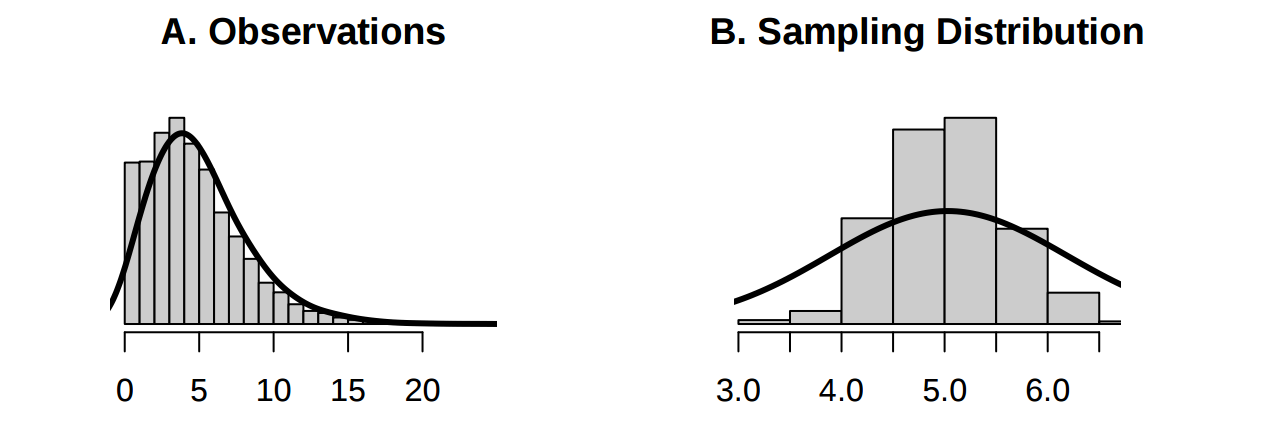
\includegraphics{exm1.png}

\subparagraph{Answer: Both are unimodal. A is right-skewed while B
appears to be left-skewed. Both are normal distributions. The means are
not equal but if more samples are used, the value might
improve.}\label{answer-both-are-unimodal.-a-is-right-skewed-while-b-appears-to-be-left-skewed.-both-are-normal-distributions.-the-means-are-not-equal-but-if-more-samples-are-used-the-value-might-improve.}

7b.Explain why the means of these two distributions are similar but the
standard deviations are not (2 pts).

\subparagraph{Answer: The means are similar because the distribution of
the mean from 500 random samples of size 30 from Observation A followed
a normal distribution (The samplings are random and the minimum number
of samples requird for normal distribution is followed). As for the
standard deviation, the distribution of the observations are farther
from the mean than in the Sampling
Distribution.}\label{answer-the-means-are-similar-because-the-distribution-of-the-mean-from-500-random-samples-of-size-30-from-observation-a-followed-a-normal-distribution-the-samplings-are-random-and-the-minimum-number-of-samples-requird-for-normal-distribution-is-followed.-as-for-the-standard-deviation-the-distribution-of-the-observations-are-farther-from-the-mean-than-in-the-sampling-distribution.}

\subparagraph{7c. What is the statistical principal that describes this
phenomenon (2
pts)?}\label{c.-what-is-the-statistical-principal-that-describes-this-phenomenon-2-pts}

\subparagraph{Answer:}\label{answer-3}

The Central Limit Theorem (CLT). All the conditions are satisfied.

The Conditions include: 1). samples are independent and random 2). Data
is not strongly skwed. 3). Distribution is approximately normal.

\section{Part II}\label{part-ii}

Consider the four datasets, each with two columns (x and y), provided
below. Be sure to replace the \texttt{NA} with your answer for each part
(e.g.~assign the mean of \texttt{x} for \texttt{data1} to the
\texttt{data1.x.mean} variable). When you Knit your answer document, a
table will be generated with all the answers.

\begin{Shaded}
\begin{Highlighting}[]
\KeywordTok{options}\NormalTok{(}\DataTypeTok{digits=}\DecValTok{2}\NormalTok{)}
\NormalTok{data1 <-}\StringTok{ }\KeywordTok{data.frame}\NormalTok{(}\DataTypeTok{x=}\KeywordTok{c}\NormalTok{(}\DecValTok{10}\NormalTok{,}\DecValTok{8}\NormalTok{,}\DecValTok{13}\NormalTok{,}\DecValTok{9}\NormalTok{,}\DecValTok{11}\NormalTok{,}\DecValTok{14}\NormalTok{,}\DecValTok{6}\NormalTok{,}\DecValTok{4}\NormalTok{,}\DecValTok{12}\NormalTok{,}\DecValTok{7}\NormalTok{,}\DecValTok{5}\NormalTok{),}
                    \DataTypeTok{y=}\KeywordTok{c}\NormalTok{(}\FloatTok{8.04}\NormalTok{,}\FloatTok{6.95}\NormalTok{,}\FloatTok{7.58}\NormalTok{,}\FloatTok{8.81}\NormalTok{,}\FloatTok{8.33}\NormalTok{,}\FloatTok{9.96}\NormalTok{,}\FloatTok{7.24}\NormalTok{,}\FloatTok{4.26}\NormalTok{,}\FloatTok{10.84}\NormalTok{,}\FloatTok{4.82}\NormalTok{,}\FloatTok{5.68}\NormalTok{))}
\NormalTok{data2 <-}\StringTok{ }\KeywordTok{data.frame}\NormalTok{(}\DataTypeTok{x=}\KeywordTok{c}\NormalTok{(}\DecValTok{10}\NormalTok{,}\DecValTok{8}\NormalTok{,}\DecValTok{13}\NormalTok{,}\DecValTok{9}\NormalTok{,}\DecValTok{11}\NormalTok{,}\DecValTok{14}\NormalTok{,}\DecValTok{6}\NormalTok{,}\DecValTok{4}\NormalTok{,}\DecValTok{12}\NormalTok{,}\DecValTok{7}\NormalTok{,}\DecValTok{5}\NormalTok{),}
                    \DataTypeTok{y=}\KeywordTok{c}\NormalTok{(}\FloatTok{9.14}\NormalTok{,}\FloatTok{8.14}\NormalTok{,}\FloatTok{8.74}\NormalTok{,}\FloatTok{8.77}\NormalTok{,}\FloatTok{9.26}\NormalTok{,}\FloatTok{8.1}\NormalTok{,}\FloatTok{6.13}\NormalTok{,}\FloatTok{3.1}\NormalTok{,}\FloatTok{9.13}\NormalTok{,}\FloatTok{7.26}\NormalTok{,}\FloatTok{4.74}\NormalTok{))}
\NormalTok{data3 <-}\StringTok{ }\KeywordTok{data.frame}\NormalTok{(}\DataTypeTok{x=}\KeywordTok{c}\NormalTok{(}\DecValTok{10}\NormalTok{,}\DecValTok{8}\NormalTok{,}\DecValTok{13}\NormalTok{,}\DecValTok{9}\NormalTok{,}\DecValTok{11}\NormalTok{,}\DecValTok{14}\NormalTok{,}\DecValTok{6}\NormalTok{,}\DecValTok{4}\NormalTok{,}\DecValTok{12}\NormalTok{,}\DecValTok{7}\NormalTok{,}\DecValTok{5}\NormalTok{),}
                    \DataTypeTok{y=}\KeywordTok{c}\NormalTok{(}\FloatTok{7.46}\NormalTok{,}\FloatTok{6.77}\NormalTok{,}\FloatTok{12.74}\NormalTok{,}\FloatTok{7.11}\NormalTok{,}\FloatTok{7.81}\NormalTok{,}\FloatTok{8.84}\NormalTok{,}\FloatTok{6.08}\NormalTok{,}\FloatTok{5.39}\NormalTok{,}\FloatTok{8.15}\NormalTok{,}\FloatTok{6.42}\NormalTok{,}\FloatTok{5.73}\NormalTok{))}
\NormalTok{data4 <-}\StringTok{ }\KeywordTok{data.frame}\NormalTok{(}\DataTypeTok{x=}\KeywordTok{c}\NormalTok{(}\DecValTok{8}\NormalTok{,}\DecValTok{8}\NormalTok{,}\DecValTok{8}\NormalTok{,}\DecValTok{8}\NormalTok{,}\DecValTok{8}\NormalTok{,}\DecValTok{8}\NormalTok{,}\DecValTok{8}\NormalTok{,}\DecValTok{19}\NormalTok{,}\DecValTok{8}\NormalTok{,}\DecValTok{8}\NormalTok{,}\DecValTok{8}\NormalTok{),}
                    \DataTypeTok{y=}\KeywordTok{c}\NormalTok{(}\FloatTok{6.58}\NormalTok{,}\FloatTok{5.76}\NormalTok{,}\FloatTok{7.71}\NormalTok{,}\FloatTok{8.84}\NormalTok{,}\FloatTok{8.47}\NormalTok{,}\FloatTok{7.04}\NormalTok{,}\FloatTok{5.25}\NormalTok{,}\FloatTok{12.5}\NormalTok{,}\FloatTok{5.56}\NormalTok{,}\FloatTok{7.91}\NormalTok{,}\FloatTok{6.89}\NormalTok{))}
\end{Highlighting}
\end{Shaded}

For each column, calculate (to two decimal places):

\paragraph{a. The mean (for x and y separately; 1
pt).}\label{a.-the-mean-for-x-and-y-separately-1-pt.}

\begin{Shaded}
\begin{Highlighting}[]
\NormalTok{(data1.x.mean <-}\StringTok{ }\KeywordTok{round}\NormalTok{(}\KeywordTok{mean}\NormalTok{(data1}\OperatorTok{$}\NormalTok{x), }\DecValTok{2}\NormalTok{))}
\end{Highlighting}
\end{Shaded}

\begin{verbatim}
## [1] 9
\end{verbatim}

\begin{Shaded}
\begin{Highlighting}[]
\NormalTok{(data1.y.mean <-}\StringTok{ }\KeywordTok{round}\NormalTok{(}\KeywordTok{mean}\NormalTok{(data1}\OperatorTok{$}\NormalTok{y), }\DecValTok{2}\NormalTok{))}
\end{Highlighting}
\end{Shaded}

\begin{verbatim}
## [1] 7.5
\end{verbatim}

\begin{Shaded}
\begin{Highlighting}[]
\NormalTok{(data2.x.mean <-}\StringTok{ }\KeywordTok{round}\NormalTok{(}\KeywordTok{mean}\NormalTok{(data2}\OperatorTok{$}\NormalTok{x), }\DecValTok{2}\NormalTok{))}
\end{Highlighting}
\end{Shaded}

\begin{verbatim}
## [1] 9
\end{verbatim}

\begin{Shaded}
\begin{Highlighting}[]
\NormalTok{(data2.y.mean <-}\StringTok{ }\KeywordTok{round}\NormalTok{(}\KeywordTok{mean}\NormalTok{(data2}\OperatorTok{$}\NormalTok{y), }\DecValTok{2}\NormalTok{))}
\end{Highlighting}
\end{Shaded}

\begin{verbatim}
## [1] 7.5
\end{verbatim}

\begin{Shaded}
\begin{Highlighting}[]
\NormalTok{(data3.x.mean <-}\StringTok{ }\KeywordTok{round}\NormalTok{(}\KeywordTok{mean}\NormalTok{(data3}\OperatorTok{$}\NormalTok{x), }\DecValTok{2}\NormalTok{))}
\end{Highlighting}
\end{Shaded}

\begin{verbatim}
## [1] 9
\end{verbatim}

\begin{Shaded}
\begin{Highlighting}[]
\NormalTok{(data3.y.mean <-}\StringTok{ }\KeywordTok{round}\NormalTok{(}\KeywordTok{mean}\NormalTok{(data3}\OperatorTok{$}\NormalTok{y), }\DecValTok{2}\NormalTok{))}
\end{Highlighting}
\end{Shaded}

\begin{verbatim}
## [1] 7.5
\end{verbatim}

\begin{Shaded}
\begin{Highlighting}[]
\NormalTok{(data4.x.mean <-}\StringTok{ }\KeywordTok{round}\NormalTok{(}\KeywordTok{mean}\NormalTok{(data4}\OperatorTok{$}\NormalTok{x), }\DecValTok{2}\NormalTok{))}
\end{Highlighting}
\end{Shaded}

\begin{verbatim}
## [1] 9
\end{verbatim}

\begin{Shaded}
\begin{Highlighting}[]
\NormalTok{(data4.y.mean <-}\StringTok{ }\KeywordTok{round}\NormalTok{(}\KeywordTok{mean}\NormalTok{(data4}\OperatorTok{$}\NormalTok{y), }\DecValTok{2}\NormalTok{))}
\end{Highlighting}
\end{Shaded}

\begin{verbatim}
## [1] 7.5
\end{verbatim}

\paragraph{b. The median (for x and y separately; 1
pt).}\label{b.-the-median-for-x-and-y-separately-1-pt.}

\begin{Shaded}
\begin{Highlighting}[]
\NormalTok{(data1.x.median <-}\StringTok{ }\KeywordTok{round}\NormalTok{(}\KeywordTok{median}\NormalTok{(data1}\OperatorTok{$}\NormalTok{x), }\DecValTok{2}\NormalTok{))}
\end{Highlighting}
\end{Shaded}

\begin{verbatim}
## [1] 9
\end{verbatim}

\begin{Shaded}
\begin{Highlighting}[]
\NormalTok{(data1.y.median <-}\StringTok{ }\KeywordTok{round}\NormalTok{(}\KeywordTok{median}\NormalTok{(data1}\OperatorTok{$}\NormalTok{y), }\DecValTok{2}\NormalTok{))}
\end{Highlighting}
\end{Shaded}

\begin{verbatim}
## [1] 7.6
\end{verbatim}

\begin{Shaded}
\begin{Highlighting}[]
\NormalTok{(data2.x.median <-}\StringTok{ }\KeywordTok{round}\NormalTok{(}\KeywordTok{median}\NormalTok{(data2}\OperatorTok{$}\NormalTok{x), }\DecValTok{2}\NormalTok{))}
\end{Highlighting}
\end{Shaded}

\begin{verbatim}
## [1] 9
\end{verbatim}

\begin{Shaded}
\begin{Highlighting}[]
\NormalTok{(data2.y.median <-}\StringTok{ }\KeywordTok{round}\NormalTok{(}\KeywordTok{median}\NormalTok{(data2}\OperatorTok{$}\NormalTok{y), }\DecValTok{2}\NormalTok{))}
\end{Highlighting}
\end{Shaded}

\begin{verbatim}
## [1] 8.1
\end{verbatim}

\begin{Shaded}
\begin{Highlighting}[]
\NormalTok{(data3.x.median <-}\StringTok{ }\KeywordTok{round}\NormalTok{(}\KeywordTok{median}\NormalTok{(data3}\OperatorTok{$}\NormalTok{x), }\DecValTok{2}\NormalTok{))}
\end{Highlighting}
\end{Shaded}

\begin{verbatim}
## [1] 9
\end{verbatim}

\begin{Shaded}
\begin{Highlighting}[]
\NormalTok{(data3.y.median <-}\StringTok{ }\KeywordTok{round}\NormalTok{(}\KeywordTok{median}\NormalTok{(data3}\OperatorTok{$}\NormalTok{y), }\DecValTok{2}\NormalTok{))}
\end{Highlighting}
\end{Shaded}

\begin{verbatim}
## [1] 7.1
\end{verbatim}

\begin{Shaded}
\begin{Highlighting}[]
\NormalTok{(data4.x.median <-}\StringTok{ }\KeywordTok{round}\NormalTok{(}\KeywordTok{median}\NormalTok{(data4}\OperatorTok{$}\NormalTok{x), }\DecValTok{2}\NormalTok{))}
\end{Highlighting}
\end{Shaded}

\begin{verbatim}
## [1] 8
\end{verbatim}

\begin{Shaded}
\begin{Highlighting}[]
\NormalTok{(data4.y.median <-}\StringTok{ }\KeywordTok{round}\NormalTok{(}\KeywordTok{median}\NormalTok{(data4}\OperatorTok{$}\NormalTok{y), }\DecValTok{2}\NormalTok{))}
\end{Highlighting}
\end{Shaded}

\begin{verbatim}
## [1] 7
\end{verbatim}

\paragraph{c. The standard deviation (for x and y separately; 1
pt).}\label{c.-the-standard-deviation-for-x-and-y-separately-1-pt.}

\begin{Shaded}
\begin{Highlighting}[]
\NormalTok{(data1.x.sd <-}\StringTok{ }\KeywordTok{round}\NormalTok{(}\KeywordTok{sd}\NormalTok{(data1}\OperatorTok{$}\NormalTok{x), }\DecValTok{2}\NormalTok{))}
\end{Highlighting}
\end{Shaded}

\begin{verbatim}
## [1] 3.3
\end{verbatim}

\begin{Shaded}
\begin{Highlighting}[]
\NormalTok{(data1.y.sd <-}\StringTok{ }\KeywordTok{round}\NormalTok{(}\KeywordTok{sd}\NormalTok{(data1}\OperatorTok{$}\NormalTok{y), }\DecValTok{2}\NormalTok{))}
\end{Highlighting}
\end{Shaded}

\begin{verbatim}
## [1] 2
\end{verbatim}

\begin{Shaded}
\begin{Highlighting}[]
\NormalTok{(data2.x.sd <-}\StringTok{ }\KeywordTok{round}\NormalTok{(}\KeywordTok{sd}\NormalTok{(data2}\OperatorTok{$}\NormalTok{x), }\DecValTok{2}\NormalTok{))}
\end{Highlighting}
\end{Shaded}

\begin{verbatim}
## [1] 3.3
\end{verbatim}

\begin{Shaded}
\begin{Highlighting}[]
\NormalTok{(data2.y.sd <-}\StringTok{ }\KeywordTok{round}\NormalTok{(}\KeywordTok{sd}\NormalTok{(data2}\OperatorTok{$}\NormalTok{y), }\DecValTok{2}\NormalTok{))}
\end{Highlighting}
\end{Shaded}

\begin{verbatim}
## [1] 2
\end{verbatim}

\begin{Shaded}
\begin{Highlighting}[]
\NormalTok{(data3.x.sd <-}\StringTok{ }\KeywordTok{round}\NormalTok{(}\KeywordTok{sd}\NormalTok{(data3}\OperatorTok{$}\NormalTok{x), }\DecValTok{2}\NormalTok{))}
\end{Highlighting}
\end{Shaded}

\begin{verbatim}
## [1] 3.3
\end{verbatim}

\begin{Shaded}
\begin{Highlighting}[]
\NormalTok{(data3.y.sd <-}\StringTok{ }\KeywordTok{round}\NormalTok{(}\KeywordTok{sd}\NormalTok{(data3}\OperatorTok{$}\NormalTok{y), }\DecValTok{2}\NormalTok{))}
\end{Highlighting}
\end{Shaded}

\begin{verbatim}
## [1] 2
\end{verbatim}

\begin{Shaded}
\begin{Highlighting}[]
\NormalTok{(data4.x.sd <-}\StringTok{ }\KeywordTok{round}\NormalTok{(}\KeywordTok{sd}\NormalTok{(data4}\OperatorTok{$}\NormalTok{x), }\DecValTok{2}\NormalTok{))}
\end{Highlighting}
\end{Shaded}

\begin{verbatim}
## [1] 3.3
\end{verbatim}

\begin{Shaded}
\begin{Highlighting}[]
\NormalTok{(data4.y.sd <-}\StringTok{ }\KeywordTok{round}\NormalTok{(}\KeywordTok{sd}\NormalTok{(data4}\OperatorTok{$}\NormalTok{y), }\DecValTok{2}\NormalTok{))}
\end{Highlighting}
\end{Shaded}

\begin{verbatim}
## [1] 2
\end{verbatim}

\paragraph{For each x and y pair, calculate (also to two decimal places;
1
pt):}\label{for-each-x-and-y-pair-calculate-also-to-two-decimal-places-1-pt}

\paragraph{d. The correlation (1 pt).}\label{d.-the-correlation-1-pt.}

\begin{Shaded}
\begin{Highlighting}[]
\NormalTok{(data1.correlation <-}\StringTok{ }\KeywordTok{round}\NormalTok{(}\KeywordTok{cor}\NormalTok{(data1), }\DecValTok{2}\NormalTok{))}
\end{Highlighting}
\end{Shaded}

\begin{verbatim}
##      x    y
## x 1.00 0.82
## y 0.82 1.00
\end{verbatim}

\begin{Shaded}
\begin{Highlighting}[]
\NormalTok{(data2.correlation <-}\StringTok{ }\KeywordTok{round}\NormalTok{(}\KeywordTok{cor}\NormalTok{(data2), }\DecValTok{2}\NormalTok{))}
\end{Highlighting}
\end{Shaded}

\begin{verbatim}
##      x    y
## x 1.00 0.82
## y 0.82 1.00
\end{verbatim}

\begin{Shaded}
\begin{Highlighting}[]
\NormalTok{(data3.correlation <-}\StringTok{ }\KeywordTok{round}\NormalTok{(}\KeywordTok{cor}\NormalTok{(data3), }\DecValTok{2}\NormalTok{))}
\end{Highlighting}
\end{Shaded}

\begin{verbatim}
##      x    y
## x 1.00 0.82
## y 0.82 1.00
\end{verbatim}

\begin{Shaded}
\begin{Highlighting}[]
\NormalTok{(data4.correlation <-}\StringTok{ }\KeywordTok{round}\NormalTok{(}\KeywordTok{cor}\NormalTok{(data4), }\DecValTok{2}\NormalTok{))}
\end{Highlighting}
\end{Shaded}

\begin{verbatim}
##      x    y
## x 1.00 0.82
## y 0.82 1.00
\end{verbatim}

\paragraph{e. Linear regression equation (2
pts).}\label{e.-linear-regression-equation-2-pts.}

\begin{Shaded}
\begin{Highlighting}[]
\NormalTok{(data1.slope <-}\StringTok{ }\KeywordTok{lm}\NormalTok{(y }\OperatorTok{~}\StringTok{ }\NormalTok{x,}\DataTypeTok{data =}\NormalTok{ data1))}
\end{Highlighting}
\end{Shaded}

\begin{verbatim}
## 
## Call:
## lm(formula = y ~ x, data = data1)
## 
## Coefficients:
## (Intercept)            x  
##         3.0          0.5
\end{verbatim}

\begin{Shaded}
\begin{Highlighting}[]
\KeywordTok{summary}\NormalTok{(data1.slope)}
\end{Highlighting}
\end{Shaded}

\begin{verbatim}
## 
## Call:
## lm(formula = y ~ x, data = data1)
## 
## Residuals:
##     Min      1Q  Median      3Q     Max 
## -1.9213 -0.4558 -0.0414  0.7094  1.8388 
## 
## Coefficients:
##             Estimate Std. Error t value Pr(>|t|)   
## (Intercept)    3.000      1.125    2.67   0.0257 * 
## x              0.500      0.118    4.24   0.0022 **
## ---
## Signif. codes:  0 '***' 0.001 '**' 0.01 '*' 0.05 '.' 0.1 ' ' 1
## 
## Residual standard error: 1.2 on 9 degrees of freedom
## Multiple R-squared:  0.667,  Adjusted R-squared:  0.629 
## F-statistic:   18 on 1 and 9 DF,  p-value: 0.00217
\end{verbatim}

\begin{Shaded}
\begin{Highlighting}[]
\NormalTok{(data2.slope <-}\StringTok{ }\KeywordTok{lm}\NormalTok{(y }\OperatorTok{~}\StringTok{ }\NormalTok{x,}\DataTypeTok{data =}\NormalTok{ data2))}
\end{Highlighting}
\end{Shaded}

\begin{verbatim}
## 
## Call:
## lm(formula = y ~ x, data = data2)
## 
## Coefficients:
## (Intercept)            x  
##         3.0          0.5
\end{verbatim}

\begin{Shaded}
\begin{Highlighting}[]
\KeywordTok{summary}\NormalTok{(data2.slope)}
\end{Highlighting}
\end{Shaded}

\begin{verbatim}
## 
## Call:
## lm(formula = y ~ x, data = data2)
## 
## Residuals:
##    Min     1Q Median     3Q    Max 
## -1.901 -0.761  0.129  0.949  1.269 
## 
## Coefficients:
##             Estimate Std. Error t value Pr(>|t|)   
## (Intercept)    3.001      1.125    2.67   0.0258 * 
## x              0.500      0.118    4.24   0.0022 **
## ---
## Signif. codes:  0 '***' 0.001 '**' 0.01 '*' 0.05 '.' 0.1 ' ' 1
## 
## Residual standard error: 1.2 on 9 degrees of freedom
## Multiple R-squared:  0.666,  Adjusted R-squared:  0.629 
## F-statistic:   18 on 1 and 9 DF,  p-value: 0.00218
\end{verbatim}

\begin{Shaded}
\begin{Highlighting}[]
\NormalTok{(data3.slope <-}\StringTok{ }\KeywordTok{lm}\NormalTok{(y }\OperatorTok{~}\StringTok{ }\NormalTok{x,}\DataTypeTok{data =}\NormalTok{ data3))}
\end{Highlighting}
\end{Shaded}

\begin{verbatim}
## 
## Call:
## lm(formula = y ~ x, data = data3)
## 
## Coefficients:
## (Intercept)            x  
##         3.0          0.5
\end{verbatim}

\begin{Shaded}
\begin{Highlighting}[]
\KeywordTok{summary}\NormalTok{(data3.slope)}
\end{Highlighting}
\end{Shaded}

\begin{verbatim}
## 
## Call:
## lm(formula = y ~ x, data = data3)
## 
## Residuals:
##    Min     1Q Median     3Q    Max 
## -1.159 -0.615 -0.230  0.154  3.241 
## 
## Coefficients:
##             Estimate Std. Error t value Pr(>|t|)   
## (Intercept)    3.002      1.124    2.67   0.0256 * 
## x              0.500      0.118    4.24   0.0022 **
## ---
## Signif. codes:  0 '***' 0.001 '**' 0.01 '*' 0.05 '.' 0.1 ' ' 1
## 
## Residual standard error: 1.2 on 9 degrees of freedom
## Multiple R-squared:  0.666,  Adjusted R-squared:  0.629 
## F-statistic:   18 on 1 and 9 DF,  p-value: 0.00218
\end{verbatim}

\begin{Shaded}
\begin{Highlighting}[]
\NormalTok{(data4.slope <-}\StringTok{ }\KeywordTok{lm}\NormalTok{(y }\OperatorTok{~}\StringTok{ }\NormalTok{x,}\DataTypeTok{data =}\NormalTok{ data4))}
\end{Highlighting}
\end{Shaded}

\begin{verbatim}
## 
## Call:
## lm(formula = y ~ x, data = data4)
## 
## Coefficients:
## (Intercept)            x  
##         3.0          0.5
\end{verbatim}

\begin{Shaded}
\begin{Highlighting}[]
\KeywordTok{summary}\NormalTok{(data4.slope)}
\end{Highlighting}
\end{Shaded}

\begin{verbatim}
## 
## Call:
## lm(formula = y ~ x, data = data4)
## 
## Residuals:
##    Min     1Q Median     3Q    Max 
## -1.751 -0.831  0.000  0.809  1.839 
## 
## Coefficients:
##             Estimate Std. Error t value Pr(>|t|)   
## (Intercept)    3.002      1.124    2.67   0.0256 * 
## x              0.500      0.118    4.24   0.0022 **
## ---
## Signif. codes:  0 '***' 0.001 '**' 0.01 '*' 0.05 '.' 0.1 ' ' 1
## 
## Residual standard error: 1.2 on 9 degrees of freedom
## Multiple R-squared:  0.667,  Adjusted R-squared:  0.63 
## F-statistic:   18 on 1 and 9 DF,  p-value: 0.00216
\end{verbatim}

\subparagraph{The intercepts:}\label{the-intercepts}

\begin{Shaded}
\begin{Highlighting}[]
\NormalTok{data1.intercept <-}\StringTok{ }\FloatTok{3.0}
\NormalTok{data2.intercept <-}\StringTok{ }\FloatTok{3.0}
\NormalTok{data3.intercept <-}\StringTok{ }\FloatTok{3.0}
\NormalTok{data4.intercept <-}\StringTok{ }\FloatTok{3.0}
\end{Highlighting}
\end{Shaded}

\subparagraph{The equations of linear
regression:}\label{the-equations-of-linear-regression}

1). data1: y = 3.000 + 0.500 * x 2). data2: y = 3.001 + 0.500 * x 3).
data3: y = 3.002 + 0.500 * x 4). data4: y = 3.002 + 0.500 * x

\paragraph{f. R-Squared (2 pts).}\label{f.-r-squared-2-pts.}

\begin{Shaded}
\begin{Highlighting}[]
\NormalTok{(data1.rsquared <-}\StringTok{ }\KeywordTok{summary}\NormalTok{(data1.slope)}\OperatorTok{$}\NormalTok{r.squared)}
\end{Highlighting}
\end{Shaded}

\begin{verbatim}
## [1] 0.67
\end{verbatim}

\begin{Shaded}
\begin{Highlighting}[]
\NormalTok{(data2.rsquared <-}\StringTok{ }\KeywordTok{summary}\NormalTok{(data2.slope)}\OperatorTok{$}\NormalTok{r.squared)}
\end{Highlighting}
\end{Shaded}

\begin{verbatim}
## [1] 0.67
\end{verbatim}

\begin{Shaded}
\begin{Highlighting}[]
\NormalTok{(data3.rsquared <-}\StringTok{ }\KeywordTok{summary}\NormalTok{(data3.slope)}\OperatorTok{$}\NormalTok{r.squared)}
\end{Highlighting}
\end{Shaded}

\begin{verbatim}
## [1] 0.67
\end{verbatim}

\begin{Shaded}
\begin{Highlighting}[]
\NormalTok{(data4.rsquared <-}\StringTok{ }\KeywordTok{summary}\NormalTok{(data4.slope)}\OperatorTok{$}\NormalTok{r.squared)}
\end{Highlighting}
\end{Shaded}

\begin{verbatim}
## [1] 0.67
\end{verbatim}

\paragraph{g. For each pair, is it appropriate to estimate a linear
regression model? Why or why not? Be specific as to why for each pair
and include appropriate plots! (4
pts)}\label{g.-for-each-pair-is-it-appropriate-to-estimate-a-linear-regression-model-why-or-why-not-be-specific-as-to-why-for-each-pair-and-include-appropriate-plots-4-pts}

\subparagraph{Answer:}\label{answer-4}

Conditions for linear regression model:

1). Linearity 2). Nearly normal residuals 3). Constant variability 4).
Observations are independent of each other

\subparagraph{data1}\label{data1}

\begin{Shaded}
\begin{Highlighting}[]
\KeywordTok{par}\NormalTok{(}\DataTypeTok{mfrow=}\KeywordTok{c}\NormalTok{(}\DecValTok{2}\NormalTok{,}\DecValTok{2}\NormalTok{))}
\KeywordTok{plot}\NormalTok{(data1, }\DataTypeTok{xlab =} \StringTok{"x"}\NormalTok{, }\DataTypeTok{ylab =} \StringTok{"y"}\NormalTok{, }\DataTypeTok{main =} \StringTok{"y vs x"}\NormalTok{)}
\KeywordTok{hist}\NormalTok{(data1.slope}\OperatorTok{$}\NormalTok{residuals, }\DataTypeTok{xlab =} \StringTok{"Residuals"}\NormalTok{, }\DataTypeTok{ylab =} \StringTok{"Frequency"}\NormalTok{, }\DataTypeTok{main =} \StringTok{"Histogram of data1 residuals"}\NormalTok{)}
\KeywordTok{qqnorm}\NormalTok{(data1.slope}\OperatorTok{$}\NormalTok{residuals)}
\KeywordTok{qqline}\NormalTok{(data1.slope}\OperatorTok{$}\NormalTok{residuals)}
\end{Highlighting}
\end{Shaded}

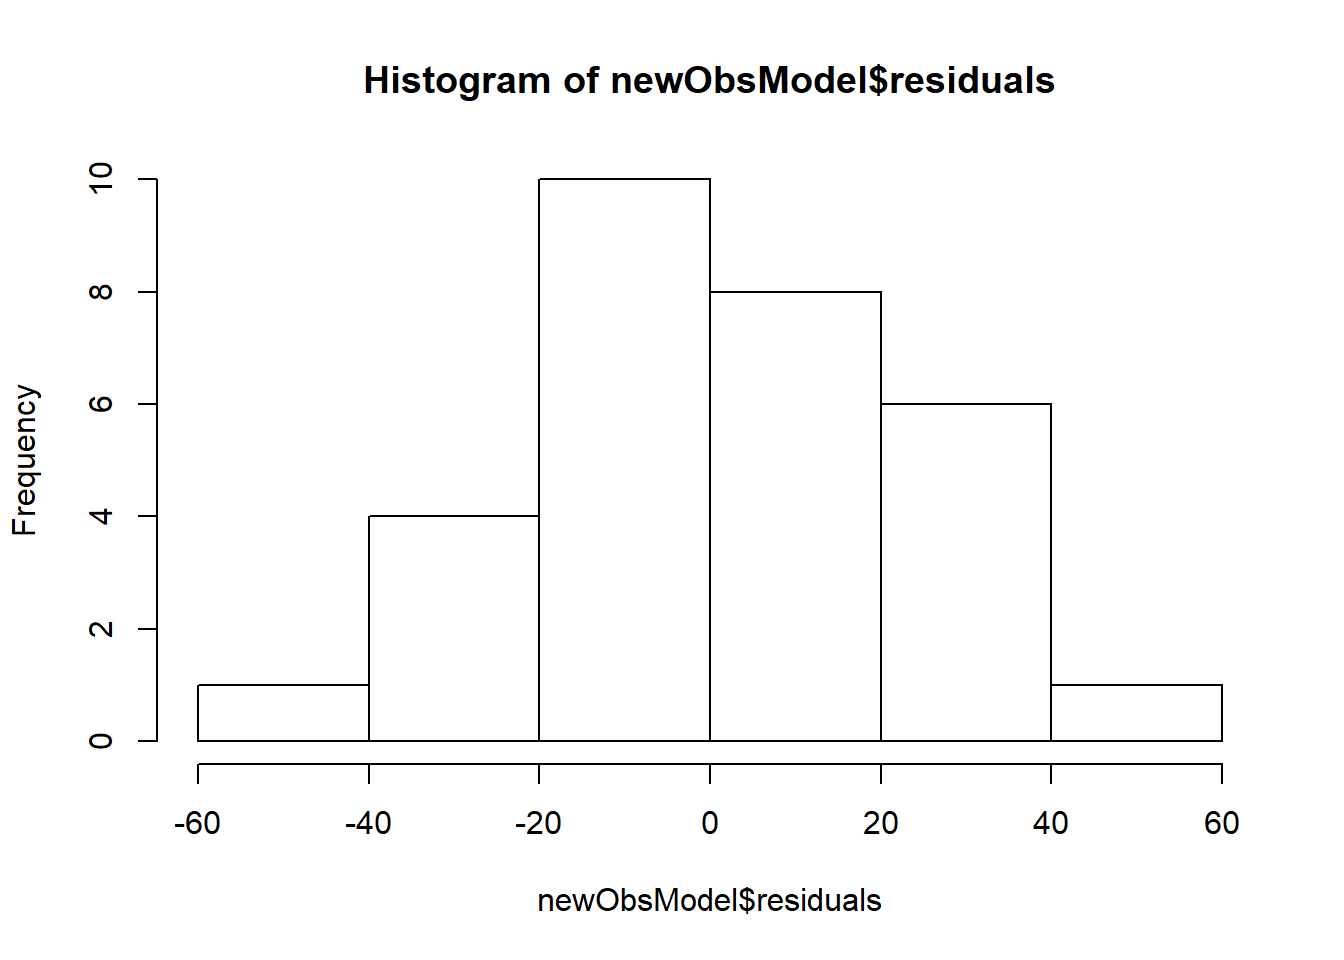
\includegraphics{Final_Exam_Answers_files/figure-latex/unnamed-chunk-16-1.pdf}

From the above plots for data1, we can see that the main plot does not
show much of linearity. While the Q-Q plot shows fairly normal
distribution with some outliers above and below the q-q line, I can't
say exactly what the nature of the histogram is. So, I will say that
linear regression model is not appropriate in this case.

\subparagraph{data2}\label{data2}

\begin{Shaded}
\begin{Highlighting}[]
\KeywordTok{par}\NormalTok{(}\DataTypeTok{mfrow=}\KeywordTok{c}\NormalTok{(}\DecValTok{2}\NormalTok{,}\DecValTok{2}\NormalTok{))}
\KeywordTok{plot}\NormalTok{(data2, }\DataTypeTok{xlab =} \StringTok{"x"}\NormalTok{, }\DataTypeTok{ylab =} \StringTok{"y"}\NormalTok{, }\DataTypeTok{main =} \StringTok{"y vs x"}\NormalTok{)}
\KeywordTok{hist}\NormalTok{(data2.slope}\OperatorTok{$}\NormalTok{residuals, }\DataTypeTok{xlab =} \StringTok{"Residuals"}\NormalTok{, }\DataTypeTok{ylab =} \StringTok{"Frequency"}\NormalTok{, }\DataTypeTok{main =} \StringTok{"Histogram of data2 residuals"}\NormalTok{)}
\KeywordTok{qqnorm}\NormalTok{(data2.slope}\OperatorTok{$}\NormalTok{residuals)}
\KeywordTok{qqline}\NormalTok{(data2.slope}\OperatorTok{$}\NormalTok{residuals)}
\end{Highlighting}
\end{Shaded}

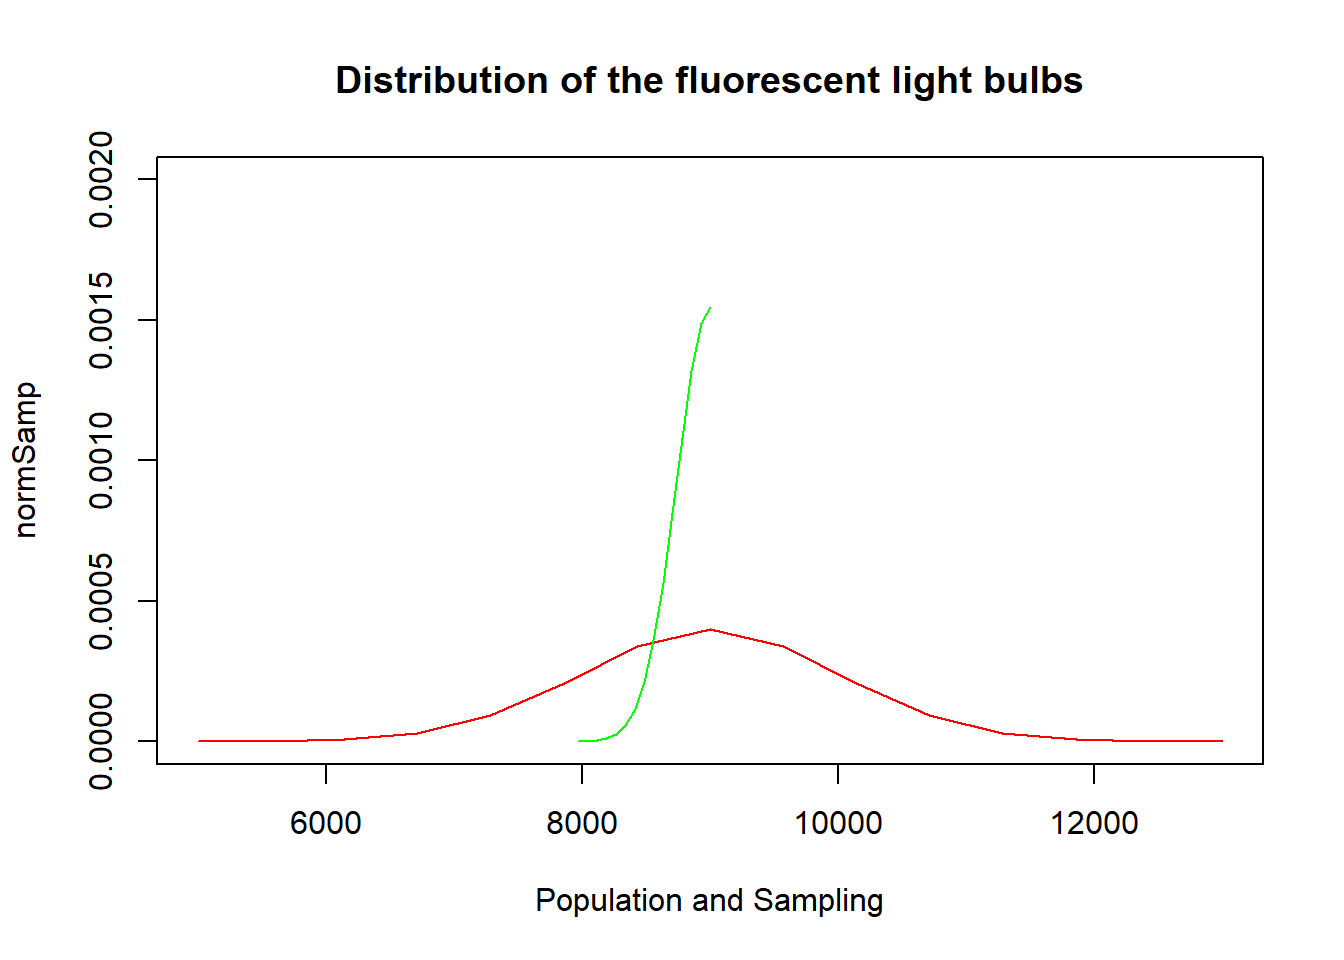
\includegraphics{Final_Exam_Answers_files/figure-latex/unnamed-chunk-17-1.pdf}

Here, we can see that the main plot has a curve which shows that it is
not linear in nature. Therefore, linear regression model will not be
appropriate.

\subparagraph{data3}\label{data3}

\begin{Shaded}
\begin{Highlighting}[]
\KeywordTok{par}\NormalTok{(}\DataTypeTok{mfrow=}\KeywordTok{c}\NormalTok{(}\DecValTok{2}\NormalTok{,}\DecValTok{2}\NormalTok{))}
\KeywordTok{plot}\NormalTok{(data3, }\DataTypeTok{xlab =} \StringTok{"x"}\NormalTok{, }\DataTypeTok{ylab =} \StringTok{"y"}\NormalTok{, }\DataTypeTok{main =} \StringTok{"y vs x"}\NormalTok{)}
\KeywordTok{hist}\NormalTok{(data3.slope}\OperatorTok{$}\NormalTok{residuals, }\DataTypeTok{xlab =} \StringTok{"Residuals"}\NormalTok{, }\DataTypeTok{ylab =} \StringTok{"Frequency"}\NormalTok{, }\DataTypeTok{main =} \StringTok{"Histogram of data3 residuals"}\NormalTok{)}
\KeywordTok{qqnorm}\NormalTok{(data3.slope}\OperatorTok{$}\NormalTok{residuals)}
\KeywordTok{qqline}\NormalTok{(data3.slope}\OperatorTok{$}\NormalTok{residuals)}
\end{Highlighting}
\end{Shaded}

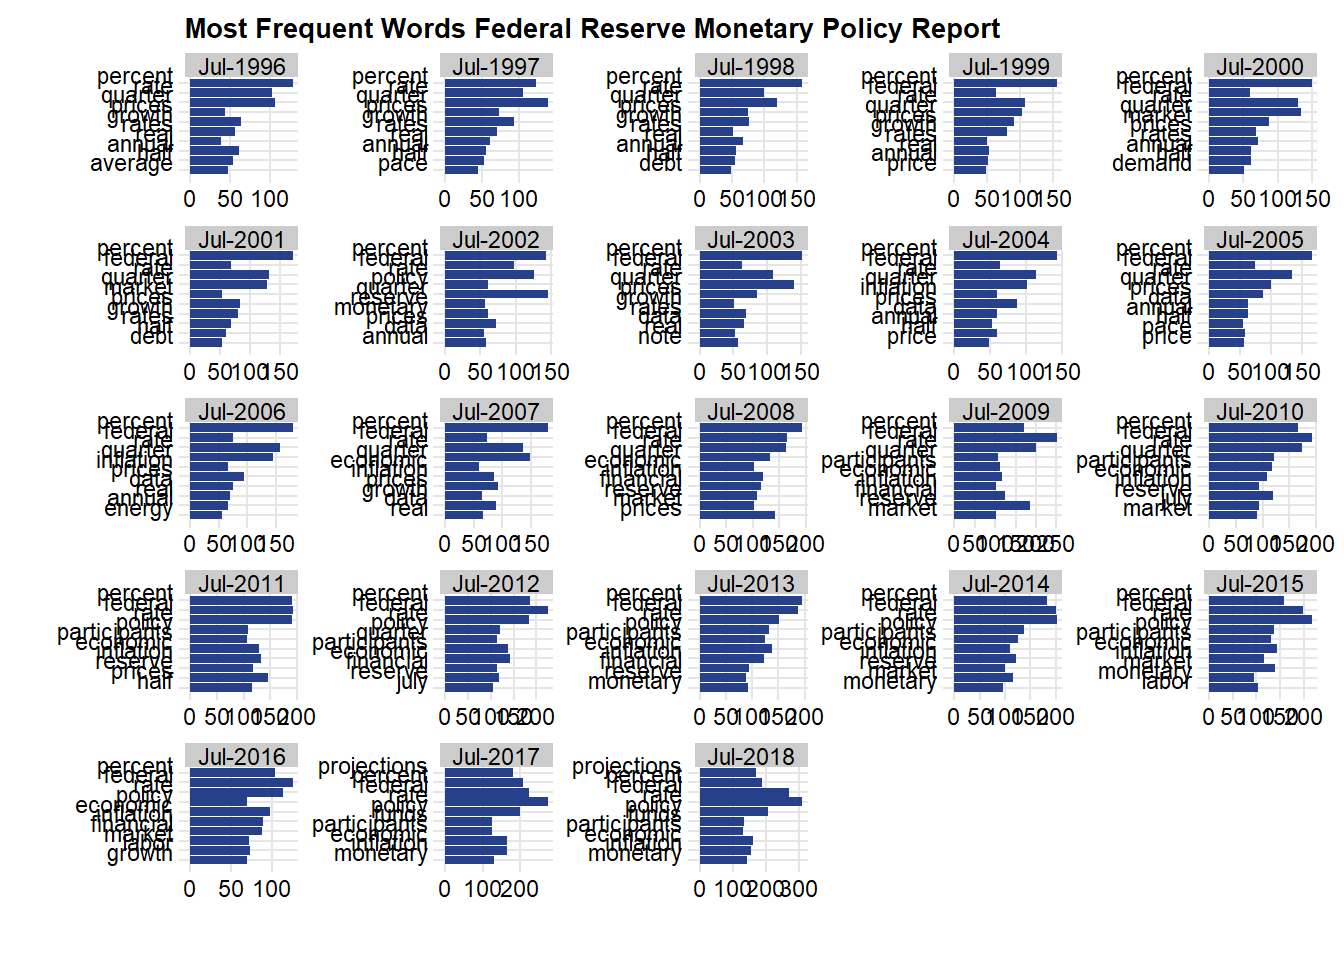
\includegraphics{Final_Exam_Answers_files/figure-latex/unnamed-chunk-18-1.pdf}

For data3, the plot shows some linearity with some outliers and the
histogram shows that distribution is approximately normal though its
output is affected by the presence of outliers.The variability of graph
changes as changes are observed in x- values.Therefore linear regression
model is not appropriate.

\subparagraph{data4}\label{data4}

\begin{Shaded}
\begin{Highlighting}[]
\KeywordTok{par}\NormalTok{(}\DataTypeTok{mfrow=}\KeywordTok{c}\NormalTok{(}\DecValTok{2}\NormalTok{,}\DecValTok{2}\NormalTok{))}
\KeywordTok{plot}\NormalTok{(data4, }\DataTypeTok{xlab =} \StringTok{"x"}\NormalTok{, }\DataTypeTok{ylab =} \StringTok{"y"}\NormalTok{, }\DataTypeTok{main =} \StringTok{"y vs x"}\NormalTok{)}
\KeywordTok{hist}\NormalTok{(data4.slope}\OperatorTok{$}\NormalTok{residuals, }\DataTypeTok{xlab =} \StringTok{"Residuals"}\NormalTok{, }\DataTypeTok{ylab =} \StringTok{"Frequency"}\NormalTok{, }\DataTypeTok{main =} \StringTok{"Histogram of data4 residuals"}\NormalTok{)}
\KeywordTok{qqnorm}\NormalTok{(data4.slope}\OperatorTok{$}\NormalTok{residuals)}
\KeywordTok{qqline}\NormalTok{(data4.slope}\OperatorTok{$}\NormalTok{residuals)}
\end{Highlighting}
\end{Shaded}

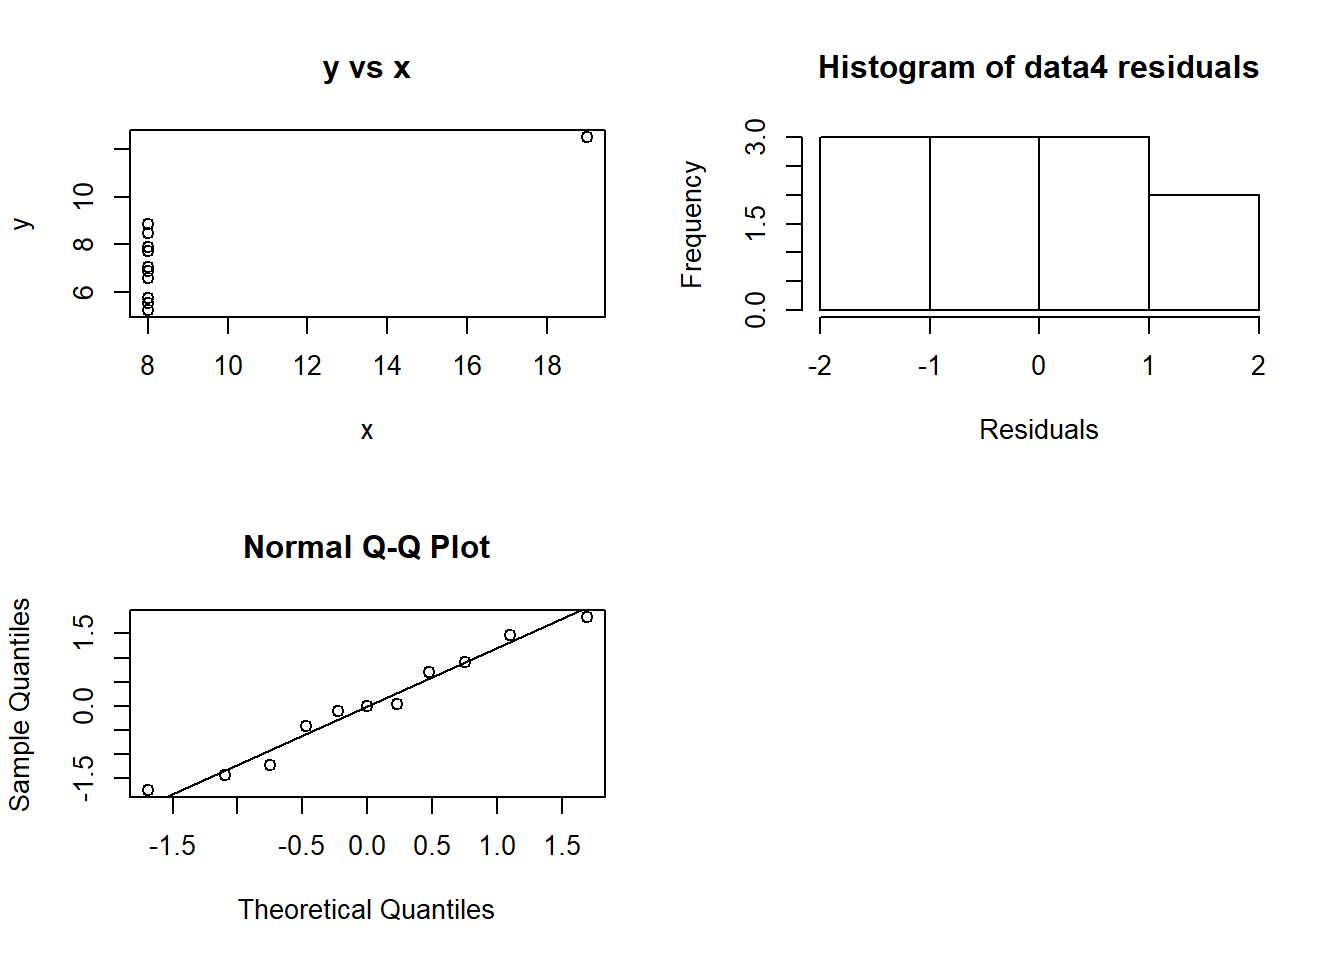
\includegraphics{Final_Exam_Answers_files/figure-latex/unnamed-chunk-19-1.pdf}

For data4, the main plot does not have linear relationship and the
histogram for residuals does not show normal distribution. So, linear
regression model will not be appropriate.

\paragraph{h. Explain why it is important to include appropriate
visualizations when analyzing data. Include any visualization(s) you
create. (2
pts)}\label{h.-explain-why-it-is-important-to-include-appropriate-visualizations-when-analyzing-data.-include-any-visualizations-you-create.-2-pts}

\subparagraph{It is important to include visualisations when analysing
data
because}\label{it-is-important-to-include-visualisations-when-analysing-data-because}

1). They help us to identify outliers in the model 2). They serve as the
first provider of insight in a snapshot into the nature of the data set
3). They help us to build conclusions and prediction about the data set
4). They help convey the result to an ordinary reader (a layman) in the
most easily presentable form.


\end{document}
